\subsection{Retrieving Model Equations -- NPZ Case Study}


Analysis of the NPZ validation study revealed that LEMMA achieved strong success in recovering both quantitative fit and ecological structure. The best-performing GPT-5 population reached an objective value of 0.0035 within three generations while maintaining a normalized ecological score of 0.676 (total score = 6.08). One other population converged (objective = 0.0069; normalized ecological score = 0.731), and several additional populations achieved objectives below 0.04 (e.g., 0.0233 and 0.0348), indicating robust predictive accuracy across multiple runs.

Ecological fidelity was consistently high across LLM families. Normalized ecological scores ranged from 0.500 to 0.898, with GPT-5 producing the highest ecological score observed (0.898; total score = 8.08). A score of 0.898 indicates that the model recovered approximately six mechanisms perfectly and provided strong alternatives for the remaining three. Median ecological scores were similar across families (Sonnet-4.5: 0.565; Gemini-2.5-pro: 0.620; GPT-5: 0.731), suggesting that most models captured key ecological processes such as phytoplankton growth and zooplankton dynamics.

\begin{figure}[H]
\centering
\includegraphics[width=\textwidth]{../Figures/NPZ_combined_with_icons.png}
\caption{Performance and ecological dynamics of NPZ model retrieval. (A) Training progress showing objective value trajectories across generations (log-scale) for GPT-5, Sonnet-4.5, and Gemini-2.5-pro. GPT-5 achieved the lowest objective value (0.0035) within three generations. (B) Time-series comparison of nutrient, phytoplankton, and zooplankton concentrations (g C m\textsuperscript{-3}) between ground-truth (black lines) and predictions from the best model by objective value (crosses). The model successfully reproduced bloom timing, nutrient drawdown, and trophic phase relationships, indicating strong alignment with ecological mechanisms.}
\label{fig:npz_timeseries}
\end{figure}

A detailed mechanism-level analysis revealed substantial variation in recovery success across NPZ processes. None of LEMMA's models perfectly recovered all of the specific ecological mechanisms in the source model from \cite{edwards1999zooplankton}, however all of the mechanisms were recovered at some point by at least one of the indiviuals (Figure~\ref{fig:mechanism_recovery}). GPT-5 consistently outperformed other LLM families, achieving the highest counts of truth matches (score = 3) for mechanisms such as phytoplankton growth and zooplankton mortality. Sonnet-4.5 and Gemini-2.5-pro often produced alternative or non-standard formulations (scores = 1-2), particularly for nutrient recycling and phytoplankton grazing loss. Mechanisms related to mixing and recycling were the most challenging across all models, with frequent absent or mistaken formulations (score = 0). These patterns suggest that while overall ecological fidelity was high, certain processes, like phytoplankton and nutrient mixing were often difficult (but not impossible) for LLMs to reconstruct accurately.

The best-performing models achieved objective values as low as 0.0035, demonstrating strong predictive accuracy while maintaining meaningful ecological structure. A detailed analysis of individual ecological characteristics (see Figure~\ref{fig:ecological_characteristics} in Supplementary Materials) revealed that some mechanisms were more readily recovered than others.

\begin{figure}[H]
\centering
\includegraphics[width=\textwidth]{../Figures/ecology_mechanism.png}
\caption{Mechanism-level recovery of NPZ equations across LLM families. Each panel shows the distribution of raw scores for a specific ecological mechanism, where 0 = absent, 1 = present (non-standard), 2 = alternative version, and 3 = truth match. Colors represent different LLM families: Sonnet-4.5, Gemini-2.5-pro, and GPT-5. GPT-5 achieved the highest frequency of truth matches for key processes such as phytoplankton growth and zooplankton mortality, while mechanisms involving nutrient recycling and mixing were most frequently absent or represented by alternative formulations.}
\label{fig:mechanism_recovery}
\end{figure}

\subsection{COTS Case Study}
\label{sec:cots_data}
For all tested LLMs, LEMMA was able to generate ecosystem models with prediction accuracy approaching the quantitative fit of the expert-developed model (objective value NMSE: 0.2312). After ten generations, objective values across LLMs (based on three independent runs per model) were as follows: GPT-5 achieved the best performance, with objective values ranging from 0.31-0.45 (lower is better), followed by Sonnet-4.5 (0.33-0.44) and Gemini-2.5-pro (0.47-0.69). Component-specific analysis revealed varying levels of prediction accuracy, with models showing strongest performance in predicting fast-growing coral cover and slow-growing coral cover, while maintaining reasonable accuracy for the more volatile COTS abundance patterns (Figure~\ref{fig:llm_comparison}). GPT-5 was able to correctly model the outbreaks of COTS, as requested in the initial prompt, while Gemini-2.5 Pro's best model was out of phase and Sonnet-4.5's identified the first, but not the second. 

The best-performing models generated by GPT-5, Claude Sonnet 4.5, and Gemini 2.5 Pro exhibited differences in structural design and ecological mechanisms, whilst also sharing several elements. GPT-5 aligned most closely with the demographic logic of the human reference model, while Gemini and Claude adopted more simplified, outbreak-oriented frameworks. Across all LLMs, certain core features remained consistent: density-dependent population regulation in crown-of-thorns starfish (COTS), resource limitation driven by coral availability, and differential effects on fast- versus slow-growing coral species. These commonalities occurred alongside substantial variation in life-history representation, recruitment formulation, immigration handling, mortality drivers, predation dynamics, and thermal stress responses (see Supplement \ref{sec:model_comparison}).

Among the LLM-generated models, GPT-5 most closely resembled the human reference model in population structure. GPT-5 modelled crown-of-thorns starfish (COTS) using two stages, juveniles and adults, while the human model applied a more detailed age-structured approach with three classes and age-specific mortality rates. In contrast, Gemini simplified the population to a single undifferentiated compartment, and Claude used a single adult compartment supplemented by episodic recruitment pulses. For recruitment, GPT-5 incorporated a Beverton-Holt-like taper on adult abundance, modified by environmental factors and lagged immigration, which paralleled the continuous Beverton-Holt density dependence used in the human model. Gemini, on the other hand, linked recruitment to coral consumption and introduced Allee effects and temperature windows without an explicit stock-recruitment curve. Claude adopted a threshold-based pulse mechanism rather than a continuous function. GPT-5 handled immigration by integrating with recruitment and applied a temporal lag, echoing the demographic embedding seen in the human model, which introduced immigration during age-0 formation with lognormal variability. Gemini instead added immigrants directly to the adult compartment, while Claude combined immigration with favorability indices and growth multipliers, creating a compound influence on population dynamics. GPT-5 and Gemini both applied baseline mortality augmented by density-dependent feedbacks, which partially reflected the human model's approach of age-specific mortality tied explicitly to prey availability. Claude introduced a starvation multiplier instead that amplified mortality when coral cover was low. For predation, GPT-5 blended Holling Type II and Type III responses, producing low-prey refuges, whereas the human model used a sigmoid saturation curve with explicit prey-switching rules. Gemini employed a standard Holling Type II functional response, and Claude incorporated prey preference weighting rather than explicit switching.
For coral growth and thermal stress, GPT-5 penalized coral growth exponentially above a thermal threshold and included a heat-loss term, which partially mirrored the human model's use of Gaussian performance curves for growth combined with logistic bleaching mortality. Gemini restricted thermal effects to logistic bleaching only, while Claude applied linear mortality beyond stress thresholds without Gaussian modulation. Finally,
temperature effects on COTS recruitment were absent from the human model but present in all LLM implementations. GPT-5 and Gemini used Gaussian temperature functions to modulate recruitment, whereas Claude embedded temperature influences within outbreak pulses and adult growth factors.

\subsection{Evolutionary Behaviour}
There were notable differences in the behaviour and speed of convergence across all LLMs tested (Figure~\ref{sec:convergence}). The Gemini-2.5 Pro models were the fastest overall, completing ten generations in approximately 36-50 minutes, with a mean time per generation of just over four minutes. GPT-5 models showed intermediate performance, averaging about 12 minutes per generation.

Patterns of improvement also differed markedly. Sonnet-4.5 and Gemini-2.5 Pro generally produced well-functioning models early but struggled to achieve consistent gains across generations, with mean improvement rates close to zero and frequent plateaus. GPT-5 demonstrated more stable progress, including the best-performing population overall (objective value 0.0035), though most GPT-5 runs also exhibited diminishing returns after initial improvements.

\begin{figure}[H]
    \centering
    \includegraphics[width=1.0\textwidth]{../Figures/llm_predictions_comparison.png}
    \caption{Comparison of model predictions across ecosystem components. The plots show observed versus predicted values for COTS abundance, fast-growing coral cover, and slow-growing coral cover, demonstrating the models' ability to capture key ecological patterns and relationships. Objective values (obj) shown in the legend represent the normalised mean squared error for all three variables, where lower values indicate better model performance.}
    \label{fig:llm_comparison}
\end{figure}
    

\subsubsection{Temporal Hold-Out}

Because GPT-5 demonstrated the strongest overall performance, we used it as the base LLM to test whether the LEMMA framework could create models capable of predicting out-of-sample datapoints. After ten generations, we found that the best-performing model (objective value: 0.29) had a reasonable degree of out-of-sample prediction performance on the withheld test dataset, with particularly strong predictive power for fast-growing coral cover (R² = 0.81, RMSE = 2.22, MAE = 1.92). Interestingly, this was a better objective value than the previous experiments where LEMMA had access to the entire time-series.

For slow-growing coral cover, the model achieved moderate predictive accuracy (R² = 0.17, RMSE = 1.6, MAE = 1.3), effectively capturing the general declining trend while showing some deviation in precise values. COTS population predictions demonstrated strong accuracy (R² = 0.75, RMSE = 0.07, MAE = 0.05), successfully capturing the timing and magnitude of major outbreaks.

Figure~\ref{fig:validation_combined} illustrates these prediction capabilities, showing both training period performance (pre-1997) and out-of-sample predictions (1997-2005). 
The model's ability to maintain consistent error metrics (RMSE and MAE) while capturing both rapid population dynamics and slower coral cover changes suggests it successfully identified fundamental ecological relationships governing this system.

\begin{figure}[H]
\centering
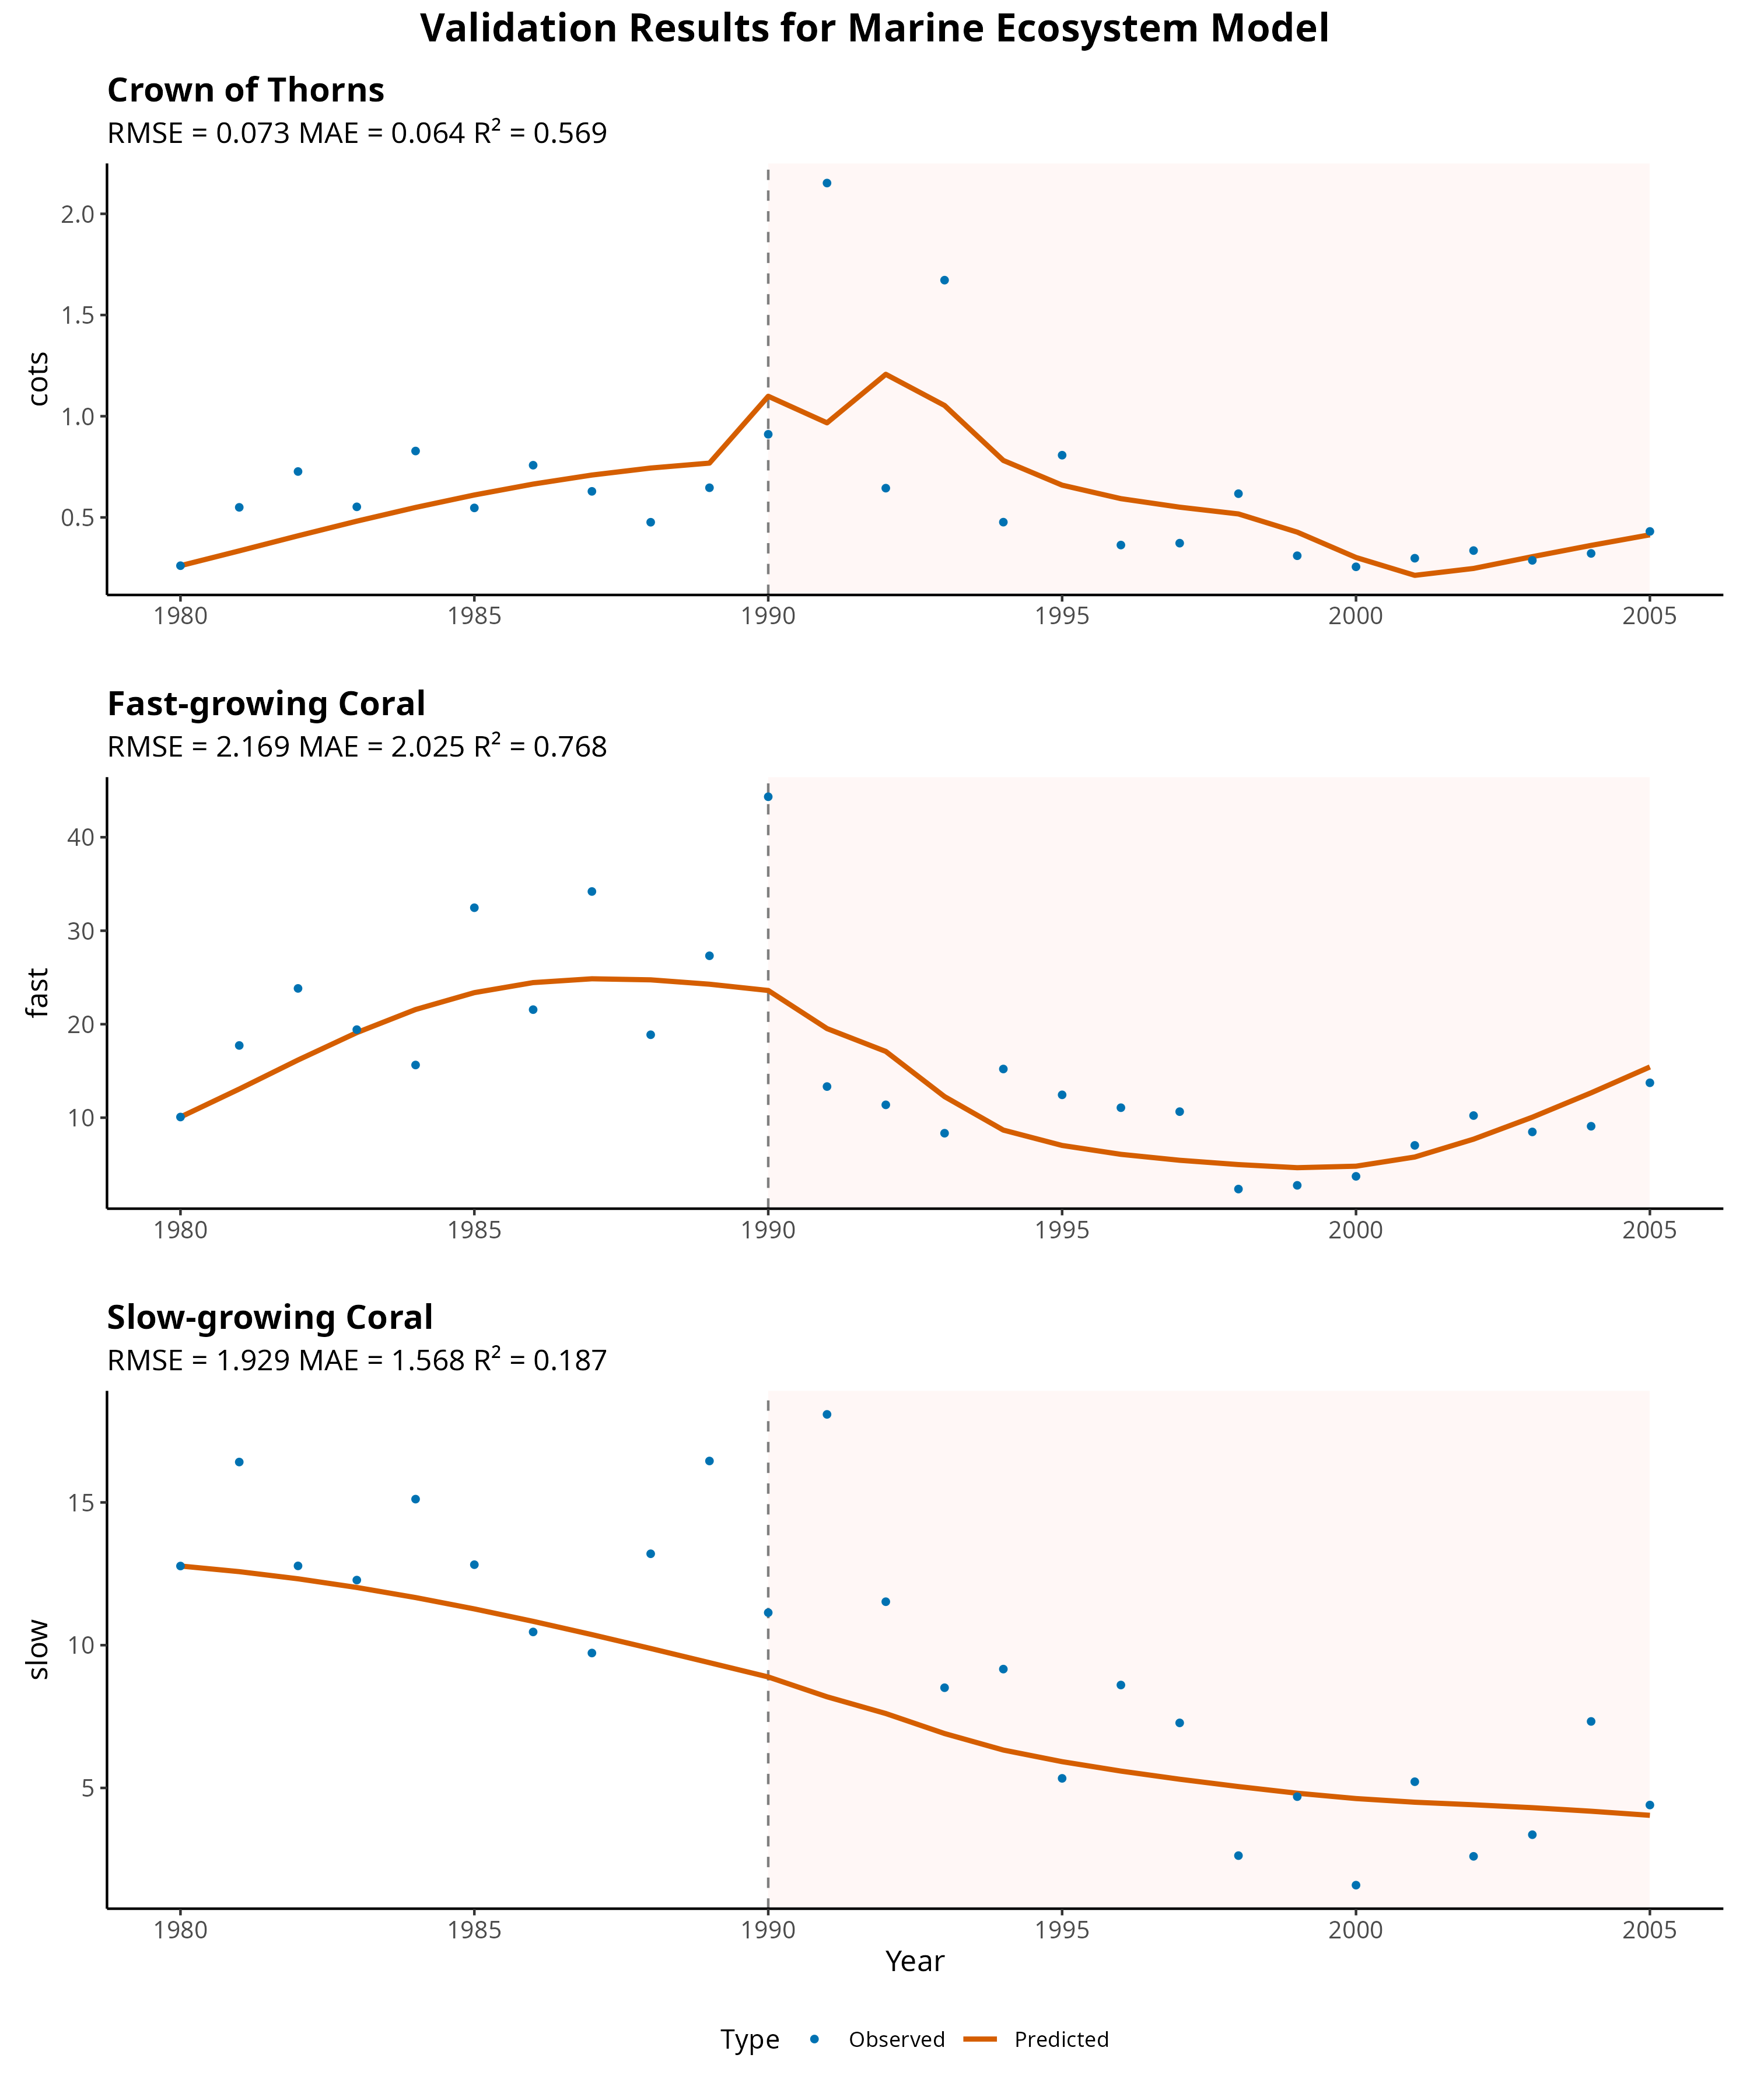
\includegraphics[width=1.0\textwidth]{../Figures/combined_validation.png}
\caption{Temporal hold-out evaluation of LEMMA driven by the best-performing LLM (GPT-5) showing predictions against observed data. LEMMA was provided with 70\% of the time-series data (pink shaded region) and developed a model that was then evaluated on the full time-series, including the remaining unseen 30\% of the time-series data (white region). Top: COTS abundance predictions showing strong capture of outbreak dynamics. Middle: Fast-growing coral cover predictions demonstrating tracking of recovery. Bottom: Slow-growing coral cover predictions illustrating general declining trends. Orange lines represent model predictions, black dots show observed data.}
\label{fig:validation_combined}
\end{figure}

\subsection{Parameter Retrieval}
\label{sec:citations_analysis}
We assessed how frequently LEMMA linked model parameters to external evidence sources, including Semantic Scholar searches and a locally curated document store. Across all generated models (21 populations, 2,619 parameters), citation integration was modest: only 3.1\% of parameters were linked to explicit citations, 1.2\% to Semantic Scholar matches, and 2.0\% to document store references. The majority of parameters lacked any external linkage.
Differences emerged between case studies. NPZ-based populations showed slightly higher citation rates (3.7\%) and semantic matches (2.7\%) than COTS-focused populations (2.8\% and 0.59\%, respectively). Document store usage was notably higher for COTS models (2.4\%) compared to NPZ (1.1\%). This disparity likely reflects the fact that the document store was curated specifically for the COTS case study, whereas no curation was performed for NPZ, limiting retrieval opportunities.
At the individual model level, citation coverage rarely exceeded 10\% of parameters, and many individuals contained no cited parameters. Where citations were present, they typically supported temperature optima, growth coefficients, and bleaching thresholds, parameters with well-documented ecological relevance. These results indicate that while LEMMA can incorporate literature-based evidence, this capability was underutilized in practice. Enhancing citation integration may require prioritizing literature-grounded parameter selection and expanding curated resources for all ecosystem contexts.
\begin{figure}[H]
\centering
\includegraphics[width=1.0\textwidth]{../Figures/citations_boxplot.png}
\caption{Distribution of citation integration across NPZ and COTS case studies. Boxplots show the percentage of parameters linked to external sources (Semantic Scholar and document store) or lacking citations. NPZ models exhibit slightly higher semantic linkage, while COTS models show greater reliance on the curated document store.}
\label{fig:citations_boxplot}
\end{figure}